\documentclass[a4paper]{article}
\usepackage{geometry}
 \geometry{
 a4paper,
 total={210mm,297mm},
 left=1.25in,
 right=1.25in,
 top=1.25in,
 bottom=1.25in,
 }
\usepackage{graphicx}
\usepackage{tgpagella}
\usepackage[T1]{fontenc}
\usepackage{titling}
\setlength{\droptitle}{-3cm}
\usepackage{subfig}

\begin{document}

\title{CS 725 Assignment 1}
\author{Sasank}
\date{\today}
\maketitle

\section{Question 1}
\begin{itemize}
\item Accuracy decreases with increase in number of neighbours. This might be because classification boundaries get less distinct.	
\item Accuracy decreases for the same reason as before. 
\begin{figure}[h]
    \centering
    \subfloat[Leave-one-out corss validation accuracy]{{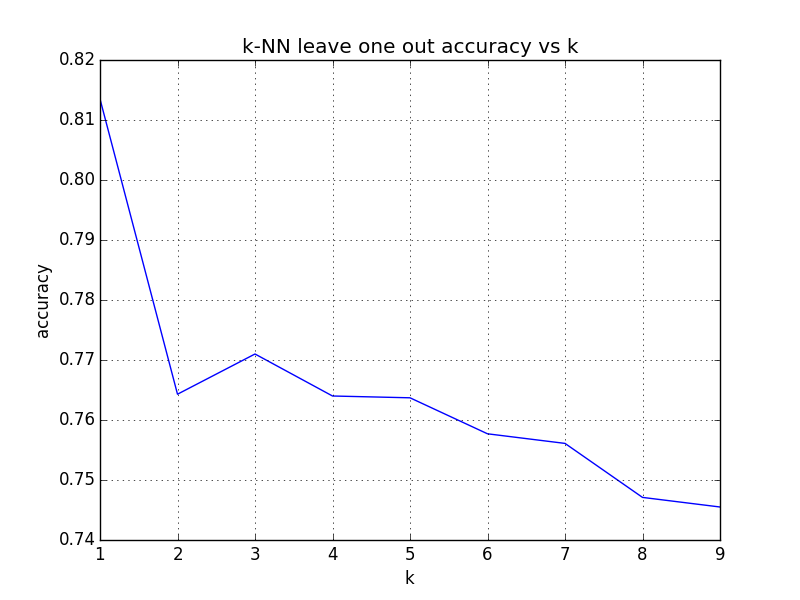
\includegraphics[width=2.5in]{q1a.png} }}%
    \qquad
    \subfloat[5-fold corss validation accuracy]{{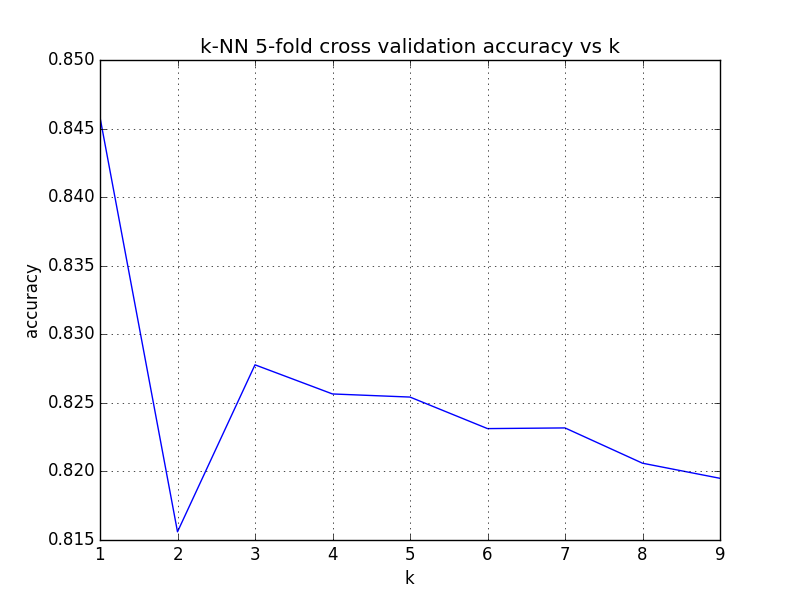
\includegraphics[width=2.5in]{q1b.png} }}%
    \label{fig:example}%
	\caption{Question 1}
\end{figure}

\end{itemize}

\section{Question 2}
In training set 1, almost all examples correspond to label $1$. In testsets $1$ and $2$, all the data correspond to labels $1$ and $2$ respectively. Thus testset1 accuracy is almost $1$ and testset2 accuracy is almost $0$.
\begin{figure}[h]
\centering
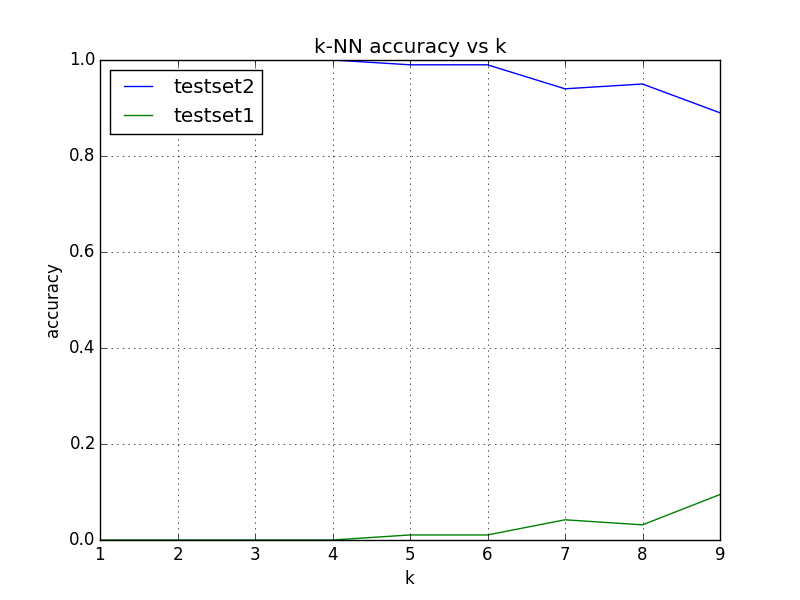
\includegraphics[width = 3.9in]{q2.png}
\caption{Question 2}
\end{figure}
\end{document}